\documentclass{article}

\usepackage{graphicx}
\usepackage{tikz}
\usepackage{tikzsymbols}
\usetikzlibrary{calc,patterns,shapes.geometric}
\pagestyle{empty}
\usepackage[margin=0pt]{geometry}
\geometry{papersize={14in,12in}}

\def\centerarc[#1](#2)(#3:#4:#5){\draw[#1] ($(#2)+({#5*cos(#3)},{#5*sin(#3)})$) arc (#3:#4:#5);}

\begin{document}
	\begin{figure}
		\centering
		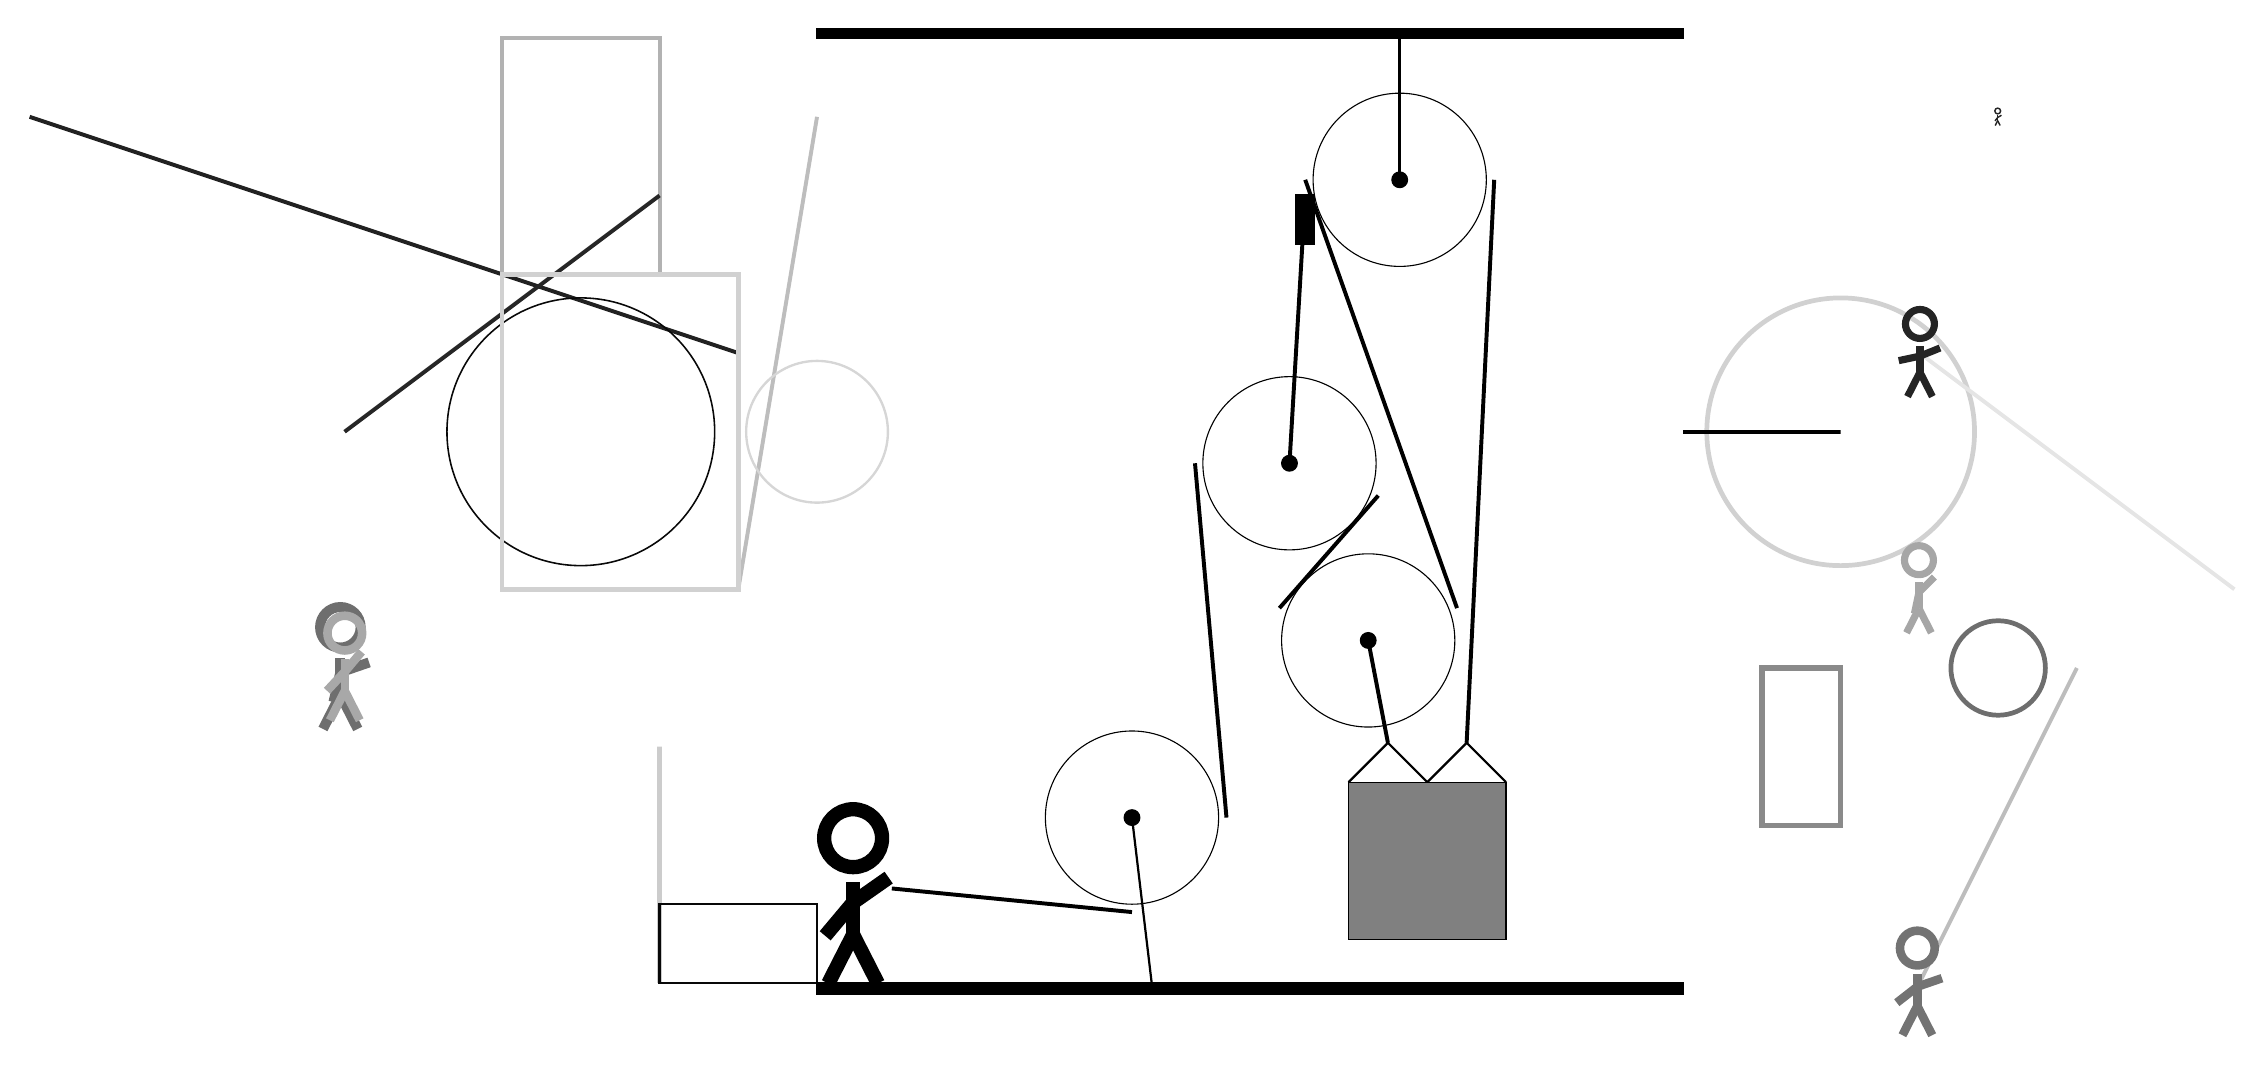
\begin{tikzpicture}
			%%%%% START %%%%%
			
			\draw[fill=black] (-6, 9) rectangle (5, 9.125);
			
			\draw (0, 3.6) circle (1.1);
			\draw[fill=black] (0, 3.6) circle (0.1);
			
			\draw (1, 1.35) circle (1.1);
			\draw[fill=black] (1, 1.35) circle (0.1);
			
			\draw (1.4, 7.2) circle (1.1);
			\draw[fill=black] (1.4, 7.2) circle (0.1);
			\draw[very thick] (1.4, 7.2) -- (1.4, 9);
			
			\draw (-2, -0.9) circle (1.1);
			\draw[fill=black] (-2, -0.9) circle (0.1);
			\draw[thick] (-2, -0.9) -- (-1.75, -3);
			
			
			\draw[thick]  (0.75, -0.45) -- (1.25, 0.05) -- (1.75, -0.45) -- (2.25, 0.05) -- (2.75, -0.45);
			\draw[fill=black!50] (0.75, -0.45) rectangle (2.75, -2.45);
			\draw[line width=0.5mm] (-5.05, -1.8) -- (-2, -2.1);
			\centerarc[line width=0.5mm](-2, -0.9)(270:360:1.2000000000000002);
			\draw[line width=0.5mm] (-0.8, -0.9) -- (-1.2, 3.6);
			\draw[line width=0.5mm] (0, 3.6) -- (0.2, 7.0);
			\draw[line width=0.5mm, fill=black](0.1, 6.4) rectangle (0.3, 7.0);
			\centerarc[line width=0.5mm](0, 3.6)(-20:180:1.2000000000000002);
			\draw[line width=0.5mm] (1.1276, 3.1896) -- (-0.1276, 1.7604);
			\centerarc[line width=0.5mm](1, 1.35)(160:380:1.2000000000000002);
			\draw[line width=0.5mm] (2.1276, 1.7604) -- (0.2, 7.2);
			\draw[line width=0.5mm](1, 1.35) -- (1.25, 0.05);
			\centerarc[line width=0.5mm](1.4, 7.2)(0:180:1.2000000000000002);
			\draw[line width=0.5mm] (2.6, 7.2) -- (2.25, 0.05);
			
			\draw[line width=0.5mm, color=black!26](-6, 8) -- (-7, 2);
			
			\draw[line width=0.7mm, color=black!20] (-8, 0) rectangle (-8, -3);
			\draw[line width=0.5mm, color=black!87](-7, 5) -- (-16, 8);
			\draw [line width=0.6mm, color=black!18](7, 4) circle (1.7);
			\node[line width=0.2mm, color=black!86] at (9, 8) {\Strichmaxerl[1][52][30]};
			\draw[line width=0.5mm, color=black!30] (-8, 9) rectangle (-10, 6);
			
			\draw[line width=0.5mm, color=black!10](8, 5) -- (12, 2);
			
			\draw[line width=0.3mm, color=black!97] (-6, -2) rectangle (-8, -3);
			\node[line width=0.5mm, color=black!57] at (-12, 1) {\Strichmaxerl[7][77][19]};
			\draw[line width=0.5mm, color=black!100] (7, 4) rectangle (5, 4);
			\draw [line width=0.3mm, color=black!16](-6, 4) circle (0.9);
			
			\draw [line width=0.2mm, color=black!97](-9, 4) circle (1.7);
			\draw[line width=0.5mm, color=black!85](-8, 7) -- (-12, 4);
			
			\draw[line width=0.5mm, color=black!26](8, -3) -- (10, 1);
			\node[line width=0.6mm, color=black!35] at (8, 2) {\Strichmaxerl[5][78][45]};
			\draw[line width=0.7mm, color=black!46] (7, 1) rectangle (6, -1);
			\node[line width=0.3mm, color=black!55] at (8, -3) {\Strichmaxerl[6][38][19]};
			\draw [line width=0.5mm, color=black!80](8, 7) circle (0.0);
			\draw [line width=0.6mm, color=black!57](9, 1) circle (0.6);
			
			\draw[line width=0.6mm, color=black!18] (-7, 6) rectangle (-10, 2);
			\node[line width=0.4mm, color=black!34] at (-12, 1) {\Strichmaxerl[6][47][50]};
			
			\node[line width=0.2mm, color=black!86] at (8, 5) {\Strichmaxerl[5][12][22]};
			
			\node at (-5.5, -1.9) {\Strichmaxerl[10][50][35]};
			
			\draw[fill=black] (-6, -3) rectangle (5, -3.15);
			
			%%%%% END %%%%%
		\end{tikzpicture}
	\end{figure}	
\end{document}